\documentclass[11pt]{article}

\usepackage{thumbpdf, amssymb, amsmath, amsthm, microtype,
	    graphicx, verbatim, listings, color, fancybox}
\usepackage[pdftex]{hyperref}
%\usepackage[margin=1in]{geometry}
\usepackage{cawsty}
\usepackage{fullpage}
\usepackage{pseudocode}

%\setlength{\parindent}{0pt}

\linespread{1.2}

\begin{document}
\arltitle{4040-849 Optimization Methods}{Written Assignment 2}
\begin{prob}{1-a}
\end{prob}
\begin{sol} 

Making the substitution of $f(\lambda)$ for $\frac{\tau_{zy}}{p_{max}}$, where $\lambda = \frac{z}{b}$, we get an equation that can be simplified as follows.

\begin{eqnarray*}
f(\lambda) & = & -\frac{1}{2}\Bigg[ -\frac{1}{\sqrt[]{1 + \lambda^2}} +  \Bigg(2 - \frac{1}{1 + \lambda^2}\Bigg) \sqrt[]{1 + \lambda^2} -2\lambda \Bigg] \\
& = & -\frac{1}{2}\Bigg[ -\frac{1}{\sqrt[]{1 + \lambda^2}} +  2\sqrt[]{1 + \lambda^2} - \frac{\sqrt[]{1 + \lambda^2}}{1 + \lambda^2} -2\lambda \Bigg] \\
& = & \frac{0.5}{\sqrt[]{1 + \lambda^2}} - \sqrt[]{1 + \lambda^2} + \frac{0.5\sqrt[]{1 + \lambda^2}}{1 + \lambda^2} + \lambda \\
& = & \frac{0.5}{\sqrt[]{1 + \lambda^2}} - \sqrt[]{1 + \lambda^2}\Bigg(1 - \frac{0.5}{1 + \lambda^2}\Bigg) + \lambda
\end{eqnarray*}

Therefore, as shown, we can reduce the problem of finding the location of the maximum shear stress for $v_{1} = v_{2} = 3$ reduces to maximizing the function shown below:

\begin{eqnarray}
\label{OriginalFunc}
f(\lambda) = \frac{0.5}{\sqrt[]{1 + \lambda^2}} - \sqrt[]{1 + \lambda^2}\Bigg(1 - \frac{0.5}{1 + \lambda^2}\Bigg) + \lambda
\end{eqnarray}

\end{sol}

\begin{prob}{1-b}
\end{prob}
\begin{sol} 

In order to apply the Fibonacci method, we must be trying to minimize the objective function for a particular problem. Therefore, since we were given an objective function (\ref{OriginalFunc}) that we must maximize, we simply negate it so that we can apply the Fibonacci method to solve it numerically. The resulting function that we seek to minimize is shown below.

\begin{eqnarray*}
f^*(\lambda) = -f\lambda) =-\frac{0.5}{\sqrt{1+\lambda^2}}+\sqrt{1+\lambda^2} \left(1-\frac{0.5}{1+\lambda^2}\right)-\lambda
\end{eqnarray*}

\begin{center}
\begin{figure}[h!]
        \label{FibFig}
        \centering
                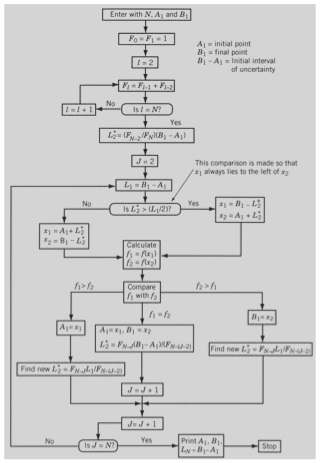
\includegraphics[width=0.5\textwidth]{fib.jpg}
        \caption{A flow diagram of the Fibonacci search method.}
\end{figure}
\end{center}

The algorithm for the Fibonacci method outlined in Figure 1 was followed with $8$, $0$, and $3$ as the initial values for $N$, $A_1$, and $B_1$, respectively, in order to manually compute the minimum of $f^*(\lambda)$ (and thus the maximum value of $f(\lambda)$). The values for $J, A_{1}, B_{1}, L_{1}, L_{2}^*$ from each of the iterations of the algorithm from $J=2$ and finishing at $J=8$ are shown below. \\

\begin{center}
  \begin{tabular}{| c | c | c | c | c | c | c | c | c | c |}
    \hline
	Step & J & $A_{1}$ & $B_{1}$ & \textbf{$L_{1}$} & \textbf{$L_{2}^{*}$} & $x_1$ & $x_2$ & $f_1$ & $f_2$\\ \hline
	1 & 2 & 0 & 3 & 3 & $\frac{39}{34}$ & $\frac{39}{34}$ & $\frac{63}{34}$ & $-0.2824$ & $-0.2223$ \\ \hline
	2 & 3 & 0 & $\frac{63}{34}$ & $\frac{63}{34}$ & $\frac{39}{34}$ & $\frac{27}{34}$ & $\frac{39}{34}$ & $-0.3000$ & $-0.2824$\\ \hline
	3 & 4 & 0 & $\frac{39}{34}$ & $\frac{39}{34}$ & $\frac{12}{17}$ & $\frac{15}{34}$ & $\frac{12}{17}$ & $-0.2631$ & $-0.2988$\\ \hline
	4 & 5 & $\frac{15}{34}$ & $\frac{39}{34}$ & $\frac{12}{17}$ & $\frac{15}{34}$ & $\frac{24}{34}$ & $\frac{15}{17}$ & $-0.2988$ & $-0.2985$\\ \hline
	5 & 6 & $\frac{15}{34}$ & $\frac{15}{17}$ & $\frac{15}{34}$ & $\frac{9}{34}$ & $\frac{21}{34}$ & $\frac{12}{17}$ & $-0.2931$ & $-0.2988$\\ \hline
	6 & 7 & $\frac{21}{34}$ & $\frac{15}{17}$ & $\frac{9}{34}$ & $\frac{3}{17}$ & $\frac{12}{17}$ & $\frac{27}{34}$ & $-0.2988$ & $-0.3003$\\ \hline
	7 & 8 & $\frac{12}{17}$ & $\frac{15}{17}$ & - & - & - & - & - & -\\ \hline
  \end{tabular}
\end{center}

The data in this table is formatted as follows:

\begin{enumerate}
	\item $A_1$ and $B_1$ - Values for $A_1$ and $B_1$ going into step (or round) $n$ of the algorithm.
	\item $L_1$ and $L_2^*$ - Values for $L_1$ and $L_2^*$ going into step (or round) $n$ of the algorithm.
	\item $x_1$ and $x_2$ - Values for $x_1$ and $x_2$ that are computed during the $n$th round of the algorithm.
	\item $f1$ and $f2$ - Values for $f_1$ and $f_2$ computed from $x_1$ and $x_2$ during the $n$th round of the algorithm.
\end{enumerate}

Once $J=N=8$ the Fibonacci algorithm is terminated and the values for $A_1 = \frac{12}{17}$ and $B_1 = \frac{15}{17}$ are displayed. Also, the value $L_n = B_1 - A_1 = \frac{3}{17} \approx 0.17647$ is returned. Note that the additional values for $L_{1}$, $L_{2}^*$, $x_1$, $x_2$, $f_1$, and $f_2$ during step $7$ were not computed because they were no longer needed in the algorithm. 

Based on the resulting interval of interest $[A_1,B_1] = [\frac{12}{17},\frac{15}{17}]$ that is returned from this algorithm, we can compute an approximate value for the maximum of $f(\lambda)$ to be $0.30027$, using $\lambda \approx \frac{A_1+B_1}{2} = \frac{12+15}{17*2} = \frac{27}{34} = 0.7941176$ as the point where the maximum occurs, which was verified to be near the maximum value for $f(\lambda)$ when computed with Mathematica.

\end{sol}

\begin{prob}{1-c}
\end{prob}
\begin{sol} 

In order to apply Newton's method to find a critical point of the given objective function (\ref{OriginalFunc}), we must derive the first and second derviatives of $f(\lambda)$ with respect to $\lambda$. The original function and its derivatives are shown below (the simplified versions of these equations were derived with the help of Mathematica and verified manually).

\begin{eqnarray*}
f(\lambda)=\frac{0.5}{\sqrt{1+\lambda^2}}-\sqrt{1+\lambda^2} \left(1-\frac{0.5}{1+\lambda^2}\right)+\lambda
\end{eqnarray*}
\begin{eqnarray*}
f'(\lambda)=\frac{\lambda \left(-\lambda^2-2\right)}{\left(\lambda^2+1\right)^{3/2}}+1 \\
\end{eqnarray*}
\begin{eqnarray*}
f''(\lambda)=\frac{\lambda^2-2}{\sqrt{\lambda^2+1} \left(\lambda^2+1\right)^2}
\end{eqnarray*}

Using these equations, we can calculate $\lambda_{i+1}$ as follows:

\begin{eqnarray*}
\lambda_{i+1} = \lambda_i - \frac{f'(\lambda_i)}{f''(\lambda_i)}
\end{eqnarray*}

Iteratively applying Newton's method with $\lambda_1 = 0.6$ as the initial point and $\epsilon=0.01$ as the termination criteria to converge towards the critical point yields the following results:

\begin{center}
  \begin{tabular}{| c | c | c | c | c |}
    \hline
	Step & $\lambda_{n}$ & $f'(\lambda_n)$ & $f''(\lambda_n)$ \\ \hline
	1 & 0.6 & 0.107199 & -0.76032 \\ \hline
	2 & 0.740991 & 0.0203098 & -0.485815 \\ \hline
	3 & 0.782797 & 0.00140041 & -0.419968 \\ \hline	
  \end{tabular}
\end{center}

The data in this table is formatted as follows:

\begin{enumerate}
	\item $\lambda_n$ - Value for $\lambda$ at step $n$ in the method.
	\item $f'(\lambda_n)$ - Value of the first derivative at $\lambda_n$.
	\item $f''(\lambda_n)$ - Value of the second derivative at $\lambda_n$. 
\end{enumerate}

By step $3$ we can see that the value of the first derivative for the given value of $f(\lambda)$ is less than $\epsilon = 0.01$ (i.e. $f'(\lambda_3) = 0.00140036 < 0.01$), so we conclude that the maximum of $f(\lambda)$ occurs at $\lambda \approx \lambda_{3} = 0.782797$, so the maximum is approximately $f(0.782797) = 0.300281$.

\end{sol}

\begin{prob}{1-d}
\end{prob}
\begin{sol} 

In order to apply the Quasi-Newton method with a fixed step size of $0.001$, we must utilize the following functions:

\begin{eqnarray}
f(\lambda) = \frac{0.5}{\sqrt[]{1 + \lambda^2}} - \sqrt[]{1 + \lambda^2}\Bigg(1 - \frac{0.5}{1 + \lambda^2}\Bigg) + \lambda
\end{eqnarray}
\begin{eqnarray*}
f^{+}(\lambda) = f(\lambda + \Delta\lambda), f^-(\lambda) = f(\lambda - \Delta\lambda)
\end{eqnarray*}
\begin{eqnarray*}
f'(\lambda) = \frac{f^{+}(\lambda) - f^{-}(\lambda)}{2\Delta\lambda}
\end{eqnarray*}
\begin{eqnarray*}
f''(\lambda) = \frac{f^{+}(\lambda) - 2f(\lambda) + f^{-}(\lambda)}{\Delta\lambda^2}
\end{eqnarray*}

Using these equations, we can calculate $\lambda_{i+1}$ as follows:

\begin{eqnarray*}
\lambda_{i+1} = \lambda_{i} - \frac{\Delta\lambda(f^{+}(\lambda_i) - f^{-}(\lambda_i))}{2(f^{+}(\lambda_i) - 2f(\lambda_i) + f^{-}(\lambda_i))}
\end{eqnarray*}

Iteratively applying the Quasi-Newton method with $\lambda_1 = 0.6$ as the initial point and $\epsilon=0.01$ as the termination criteria to converge towards the critical point yields the following results:

\begin{center}
  \begin{tabular}{| c | c | c | c | c | c | c | c | }
    \hline
	Step & $\lambda_{n}$ & $f(\lambda_n)$ & $f^{+}(\lambda_n)$ & $f^{-}(\lambda_n)$ & $f'(\lambda_n)$\\ \hline
	1 & 0.6 & 0.291303 & 0.291409 & 0.291195  & 0.107199\\ \hline	
	2 & 0.740992 & 0.299837 & 0.299857 & 0.299816 & 0.0203097\\ \hline
	3 & 0.782797 & 0.300281 & 0.300282 & 0.300279 & 0.0014006 \\ \hline
  \end{tabular}
\end{center}

The data in this table is formatted as follows:

\begin{enumerate}
	\item $\lambda_n$ - Value for $\lambda$ at step $n$ in the method.
	\item $f(\lambda_n)$ - Value of the original function at $\lambda_n$.
	\item $f^+(\lambda_n)$ - Value of the function $f^+(\lambda)$ at $\lambda_n$.
	\item $f^-(\lambda_n)$ - Value of the function $f^-(\lambda)$ at $\lambda_n$.
	\item $f'(\lambda_n)$ - Value of the second derivative at $\lambda_n$. 
\end{enumerate}

By step $3$ we can see that the value of the approximated first derivative for $f(\lambda)$ is less than or equal to the $\epsilon = 0.01$ (i.e. $f'(\lambda_3) = 0.0014006 < 0.01$), so we conclude that the maximum of $f(\lambda)$ occurs at $\lambda \approx \lambda_{3} = 0.782797$, so the maximum is approximately $f(0.782797) = 0.300281$.

\end{sol}

\end{document}
